\section{Performance Analysis}
In our tool we have developer a \textit{script} which records timestamps and duration time of big data analysis in a \texttt{.csv} file, called \texttt{PerformanceHistory.csv}. The \textit{script} mentioned before is used in order to figure out the time of analysis. 
The environment in which we tested our tool is a cluster of the University of Verona, running Ubuntu 18.04.1 LTS, it has an Intel Xeon Processor (Skylake, IBRS) and a memory of 7880 MiB. 

\begin{table}[h]
\centering
\begin{tabular}{|l|l|c|}
\hline
\textbf{Dataset} & \textbf{Description}                              & \textbf{Size} \\ \hline
no\_atk          & Traffic log in normal conditions, no attacks. & 1.3 GB        \\ 
dos\_atk         & Traffic log during a DoS attack.                   & 1.6 GB        \\ 
ddos\_atk        & Traffic log during a DDoS attack with 40 bots. & 1.6 GB        \\ \hline
\end{tabular}
\caption{Datasets Info}
\label{tab:dataset_info}
\end{table}

\begin{figure*}[h]
	\begin{subfigure}{0.48\textwidth}
		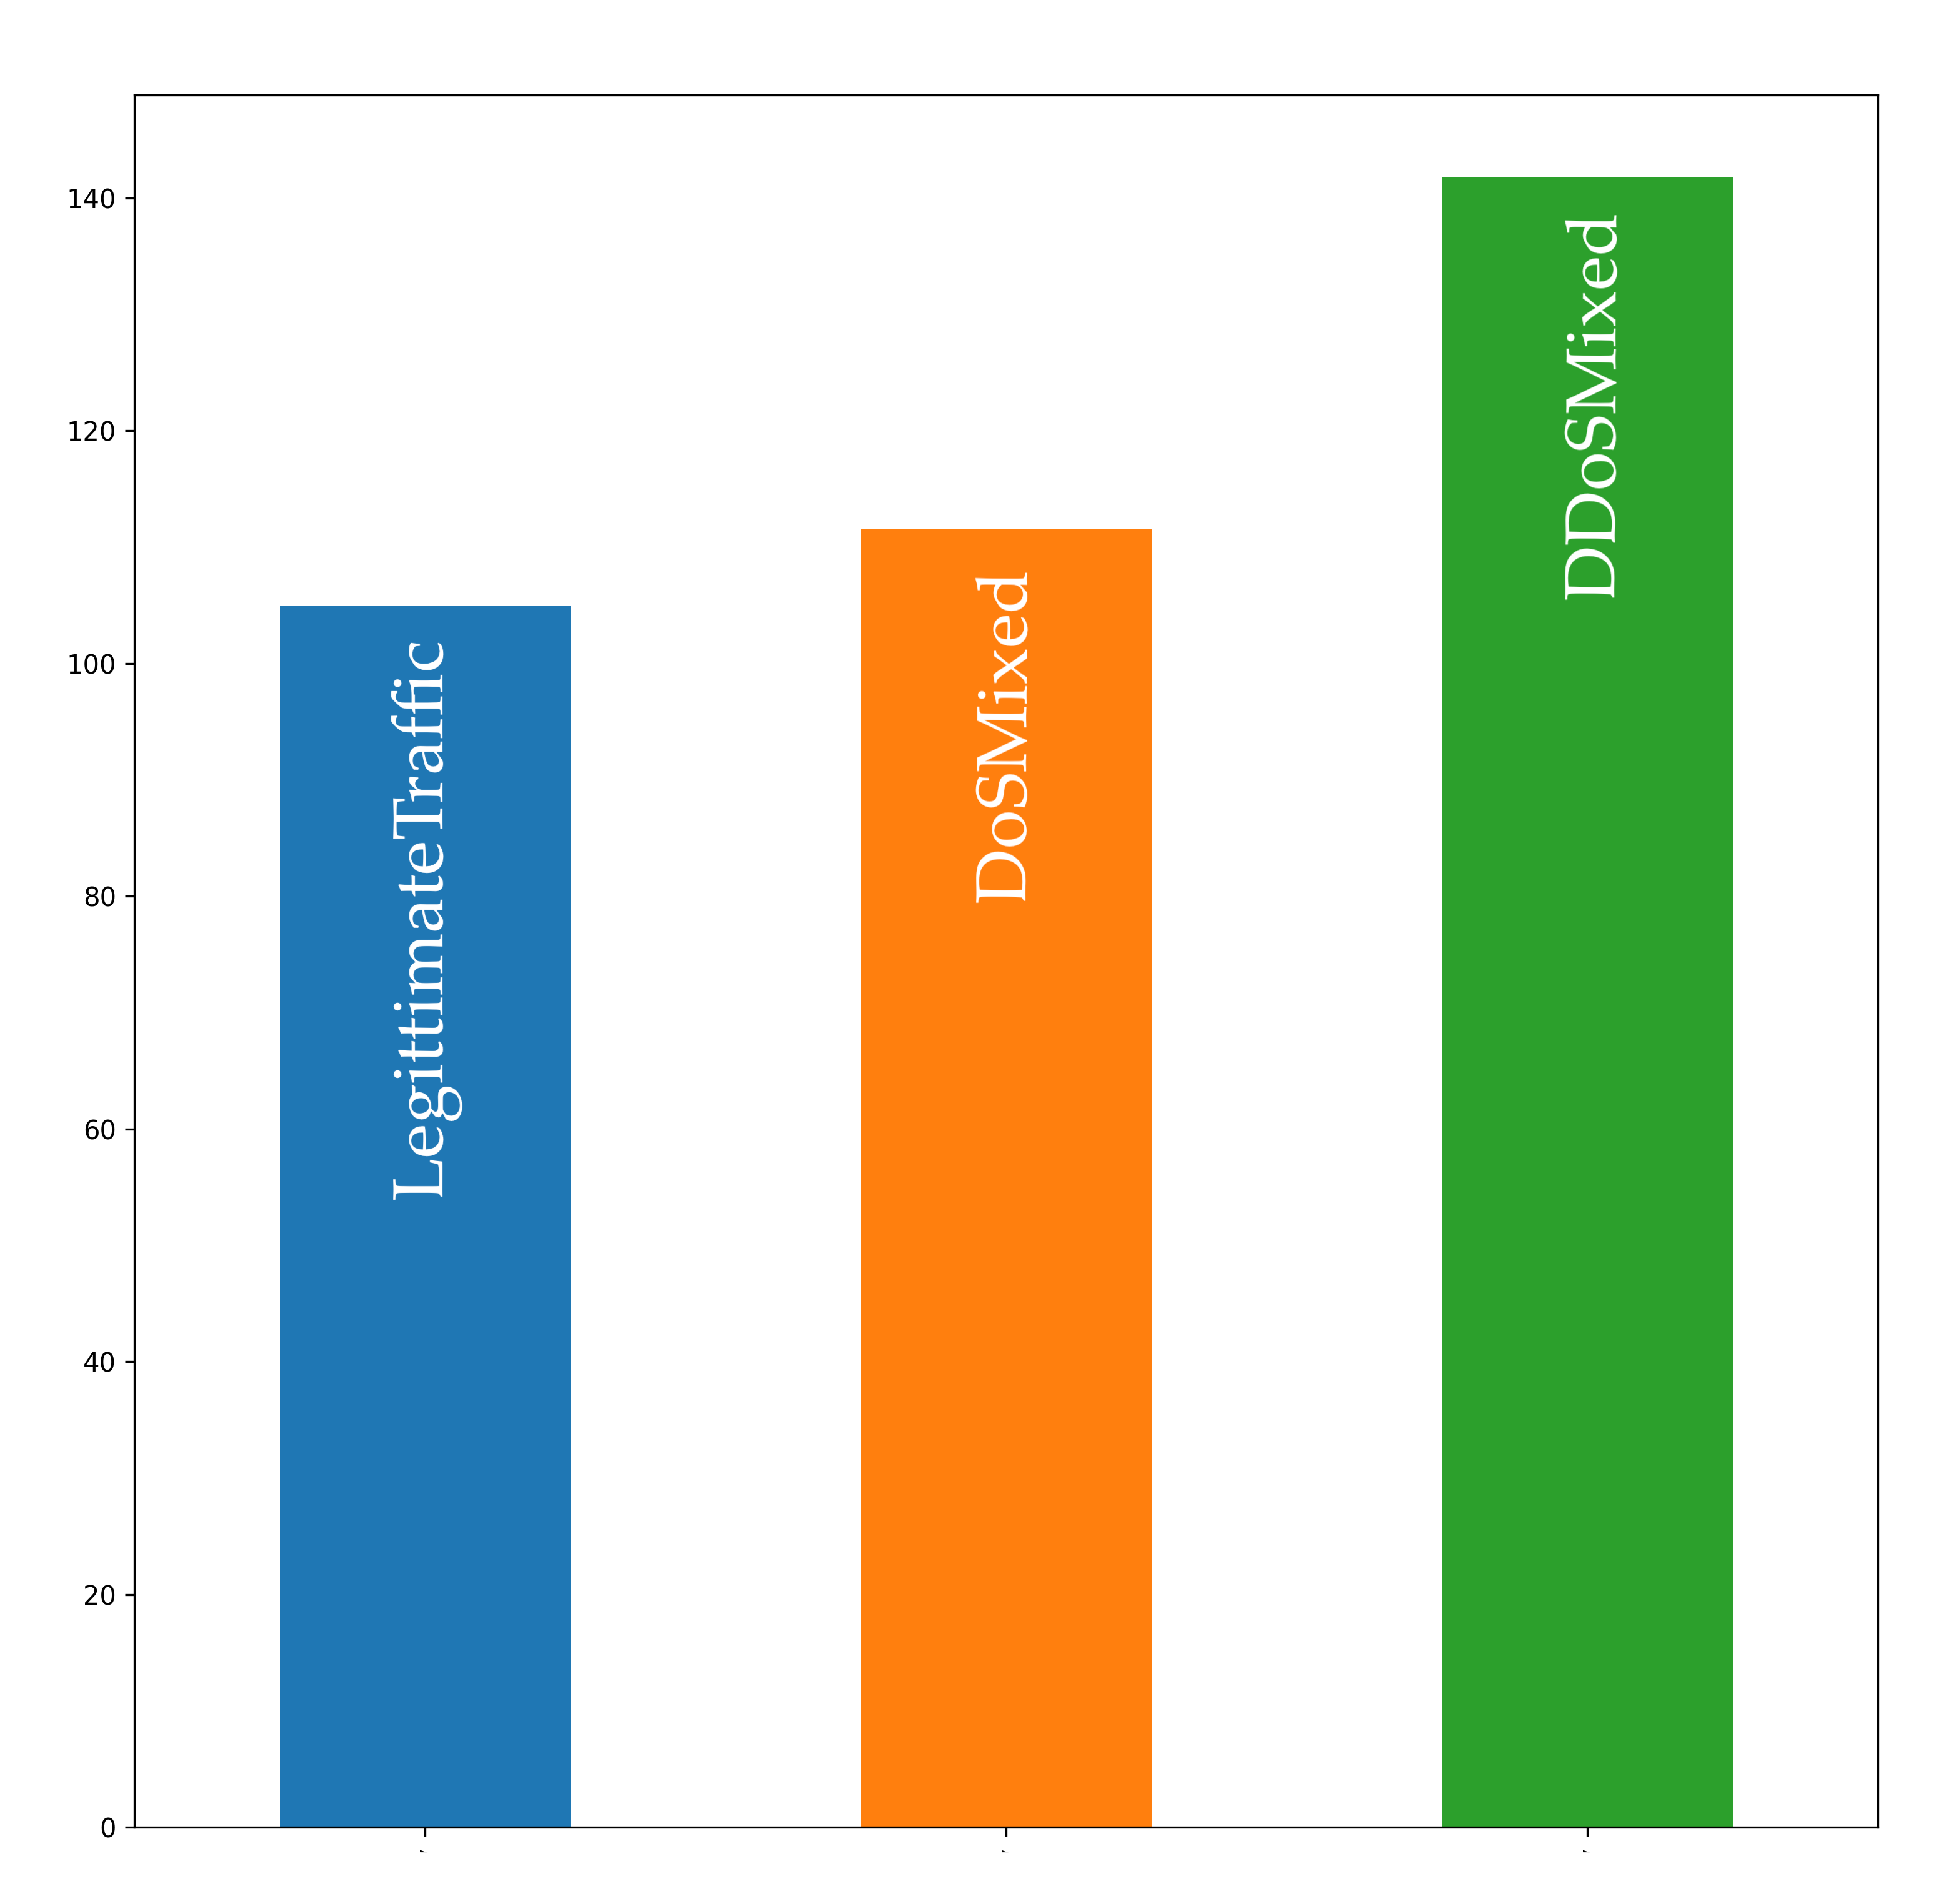
\includegraphics[width=\textwidth]{imgs/analysis_stat.png}
		\caption{Datasets analysis data statistics} 
		\label{fig:analysis_stats}
	\end{subfigure}
	\hspace*{\fill} % separation between the subfigures
	\begin{subfigure}{0.48\textwidth}
		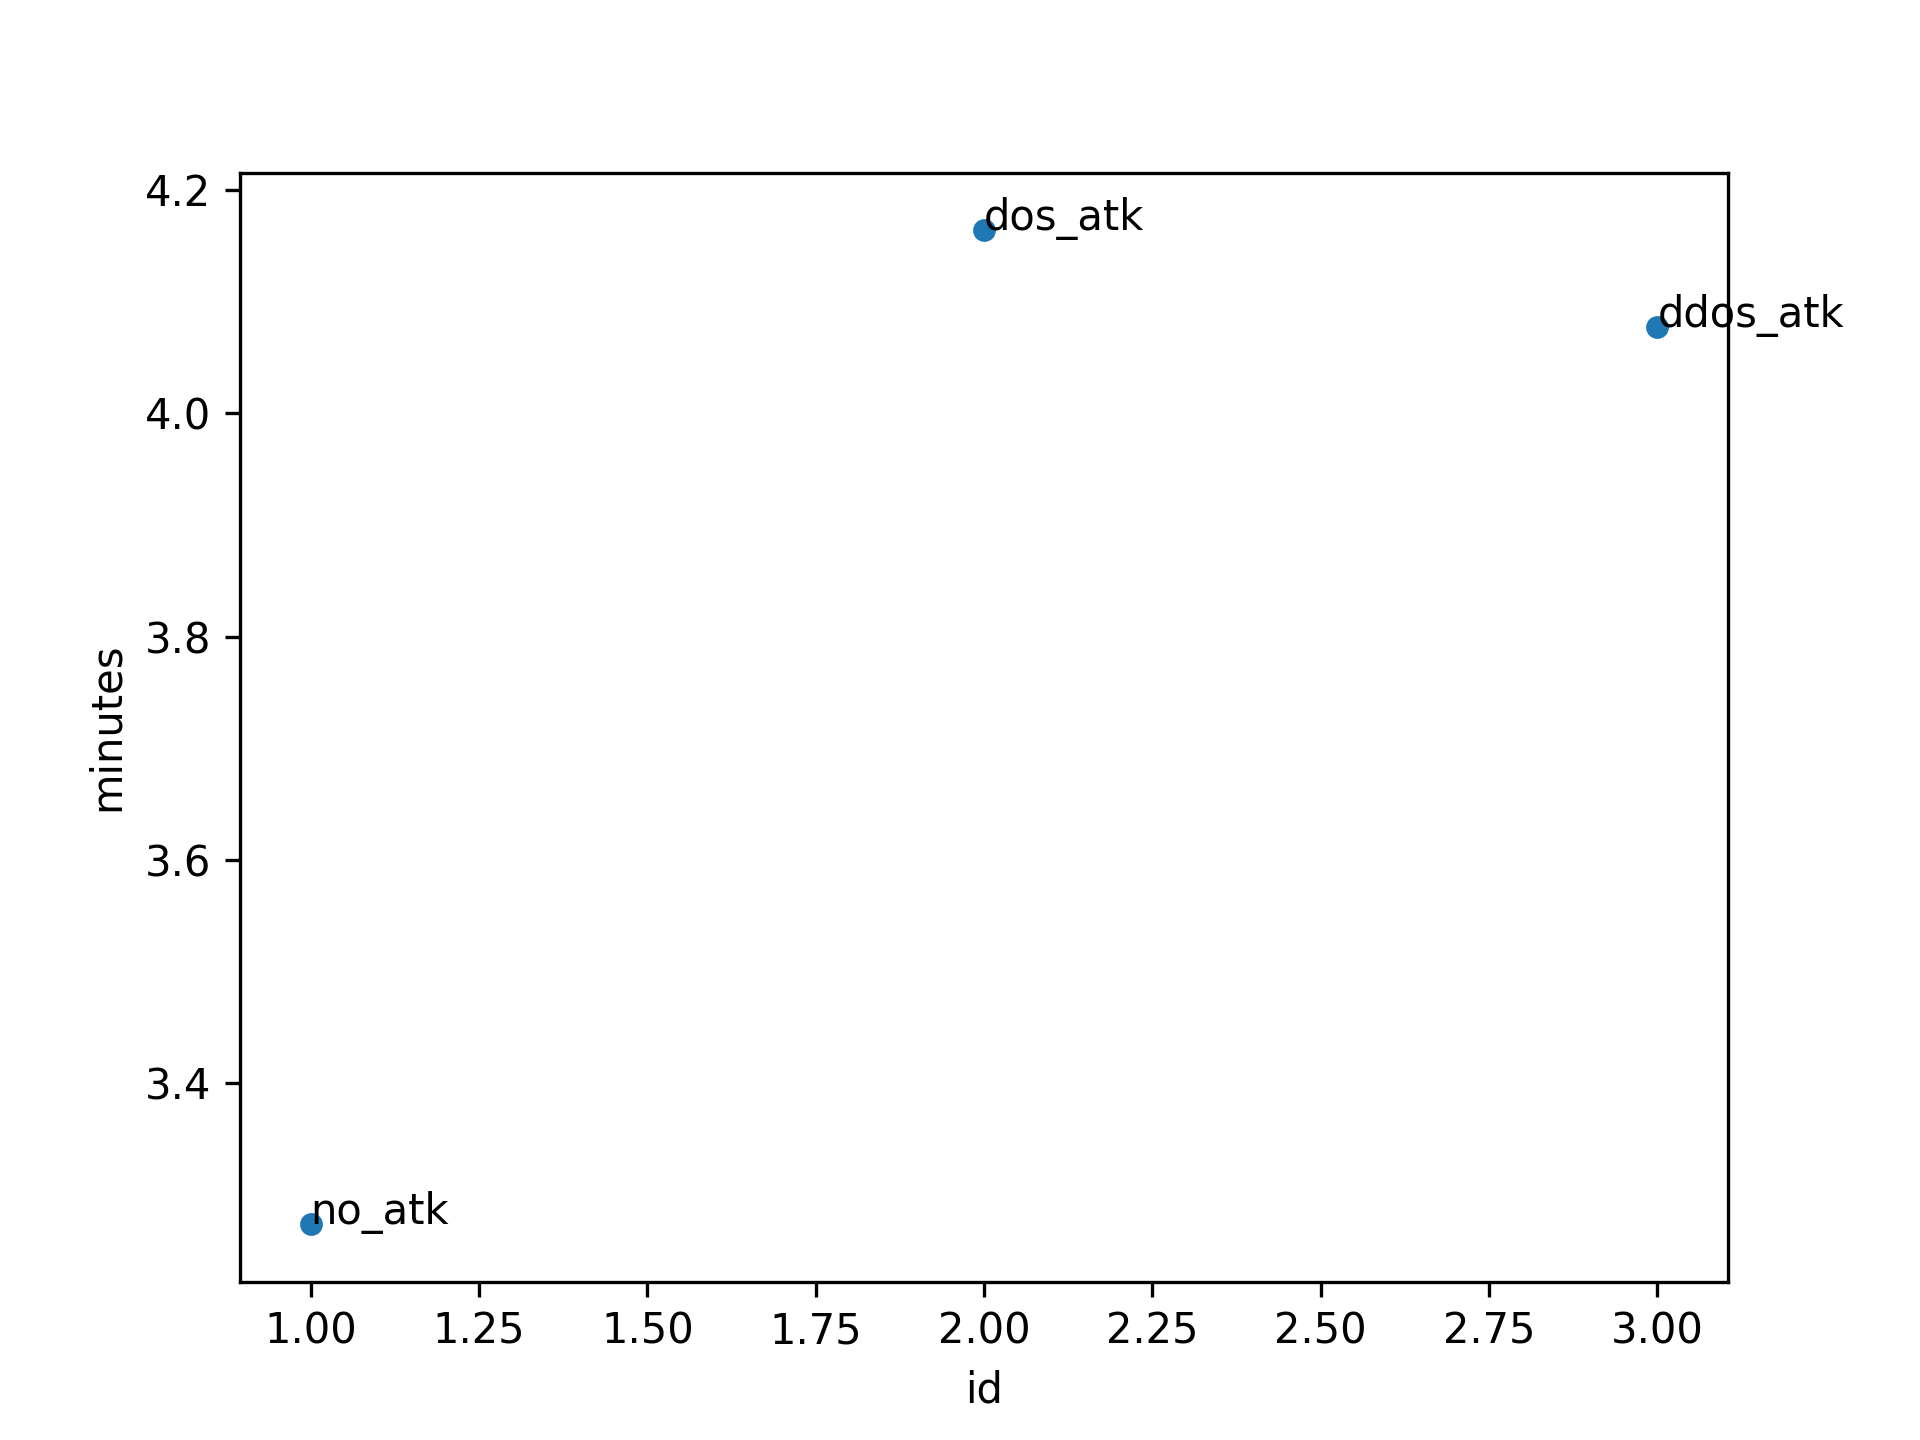
\includegraphics[width=\textwidth]{imgs/generation_stat.png}
		\caption{Datasets generation data statistics} 
		\label{fig:generation_stats}
	\end{subfigure}
	\caption{Datasets statistics}
	\label{fig:datasets_statistics}
\end{figure*}

Using our script called \texttt{PerformanceAnalysis.py} we managed to plot the time elapsed to generate and analyze the datasets listed into Tab. \ref{tab:dataset_info}: results are reported into Fig. \ref{fig:datasets_statistics}. \\
We can immediately see that the generation time is much greater for attack datasets: this is justifiable because of the greater size, considering multi-user disk accesses.
Talking about analysis statistics, we can see a spike in \textit{ddos\_atk} and \textit{no\_atk} datasets. Here, long cluster timeouts during Pig Latin script execution play a great role, and we cannot have much control over it. Without that problem, analysis of the datasets would have taken much less time.


